\documentclass[a4paper,12pt]{article}
\usepackage[slovene]{babel}
\usepackage[utf8]{inputenc}
\usepackage{multicol}
\usepackage{fullpage}
\usepackage{guitar}
\usepackage{titlesec}
\usepackage{graphicx}
\setcounter{secnumdepth}{-1} 
\usepackage[absolute]{textpos}
\titleformat{\chapter}{\large\bfseries}{\thesection}{1em}{}
\titleformat{\section}{\Large\bfseries}{\thesection}{1em}{}
\titleformat{\subsection}{\large\bfseries}{\thesection}{1em}{}

\begin{document}
\pagenumbering{Roman}
\begin{titlepage}
\begin{textblock*}{297mm}(-6mm,-0mm)
\includegraphics[width=\paperwidth]
{frontpages/2014.png}\end{textblock*} \
\end{titlepage}
\setlength{\columnseprule}{0.5pt}
\begin{multicols}{2}
\tableofcontents
\end{multicols}
\pagebreak

\setlength{\columnseprule}{0.5pt}
\begin{multicols}{2}
\pagenumbering{arabic}
\section{Akordi}
\begin{guitar}
[A - X02220  Am - X02210]

[B - X13331  Bm - X13321]

[C - X32010  Cm - X35543]  

[D - XX0232  Dm - XX0231] 

[E - 022100  Em - 022000] 

[F - 133211  Fm - 133111]

[G - 320003  Gm - 355333]

[H - X24442  Hm - X24432]


[A7 - X02020  B7 - X13131]

[C7 - X32310  D7 - XX0212]

[E7 - 020100  F7 - 131211]

[G7 - 320001  H7 - X21202]


[Am7 - X02010  Bm7 - X13121]

[Cm7 - X35343  Dm7 - XX0211]

[Em7 - 022030  Fm7 - 131111]

[Gm7 - 353333  Hm7 - X24232]


[C# - X46664  D# - 779997]

[F# - 244322  G# - 466544]


[C#m - X46654  D#m - 779987]

[F#m - 133111  G#m - 466444]


[A6 - X02222  C6 - X055555]

[D6 - X077777 E6 - X099999]


[ASUS2 - X02200]

[ASUS4 - X02230]

[DSUS2 - XX0320] 

[DSUS4 - XX0233]

[ESUS4 - 022200]

[CMAJ7 - X32000]

[FMAJ7 - 103210]

[GMAJ7 - 3X0032]

[DADD4/ADD2 - 554030]

\end{guitar}
\subsection*{Barre akordi}
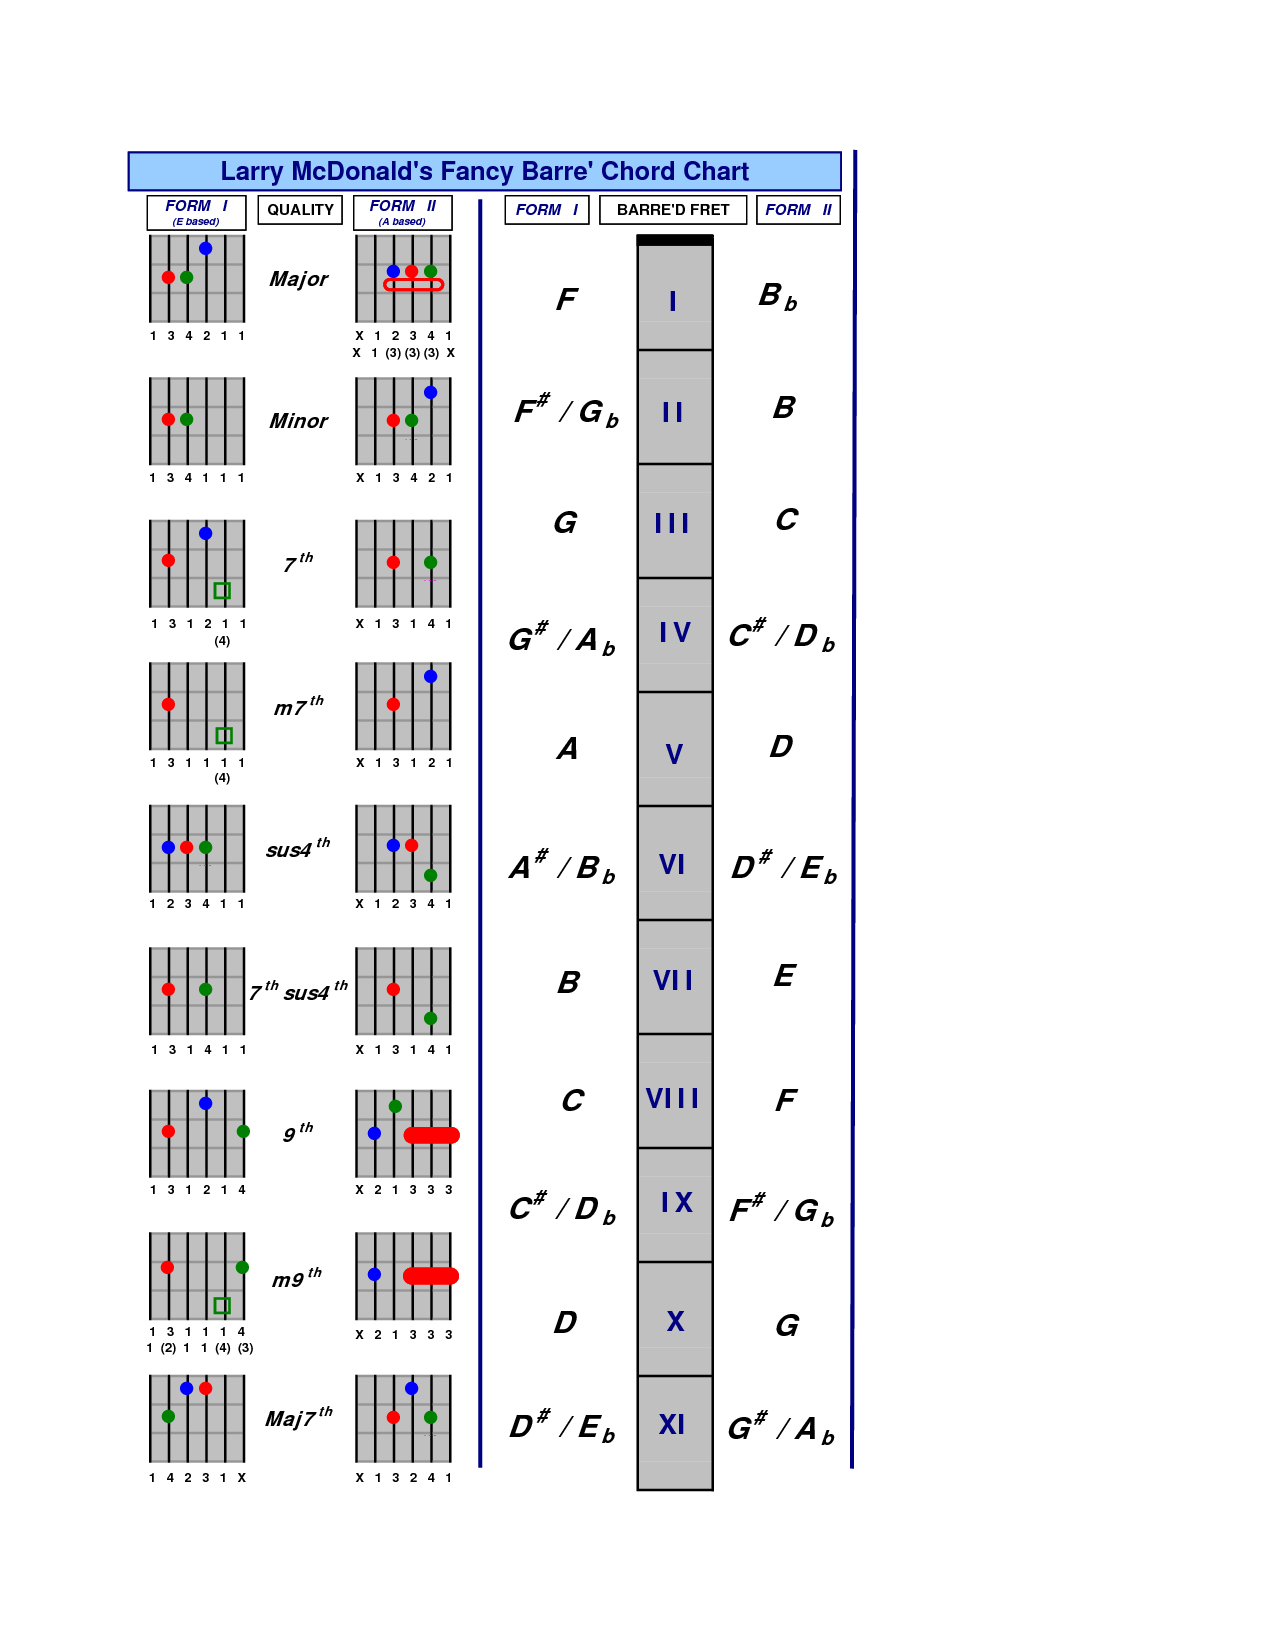
\includegraphics[width=140mm]{img/barre.png}
\clearpage
\section{Adijo knapi}
\subsection*{Orleki}
\begin{guitar}
[F Am B F]

[F]Samo nekaj let je [Am]se ostalo,
in [B]gverk se bo za[F]prl,
za njim ostal bo spome[Am]nik na trgu
in ob [B]njem zarustan [F]hunt,
donferca ne [Am]bo vozila,
[B]kolma na šta[F]cjon,
ampak bo utruje[Am]na krasila
[B]nov ajzen[F]pon.


[Dm]Dvesto let je [Am]rod za rodom [B]grizel v to zem[F]ljo,
[Dm]Dvesto let je [Am]rod za rodom 
[B]preklinjal pod [F]zemljo.


Pesem krampov bo zamrla
in kamerati se bojo razšli,
nekam v kot v muzej se bo zadigal
v štil popljuvan herc.
Kdo odslej bo štrajke delal
in kdo frdinste klel
kdo odslej bo fano nosil
ko kak hajer bo umrl.


Dvesto let je rod za rodom grizel v to zemljo,
dvesto let je rod za rodom 
preklinjal pod zemljo.


Dvesto let...


Skozi vašhav bo le vahtar hodil,
skoz gezenke bo vleku prepih,
nihče ne bo več huntov rajdal
in nihče po hofu klel,
pesem krampov bo zamrla
in kamerati se bojo razšli
in ko se zadnji zajbrovc bo na britof znajdu
z njim umrl bo še spomin.


Dvesto let..
\end{guitar}
\end{multicols}
\clearpage
\clearpage
\null
\vfill
\center

\includegraphics[width=100px]{img/licence.png}

Pesmarica je zaščitena z licenco CC-BY-NC-SA. Vse pesmi so delo in last avtorjev. Morebitne napake in predloge sporočite na pesmarica.info@gmail.com 

Izvorna koda (LaTeX) ter PDF sta dostopna na https://github.com/gztproject/Pesmarica
\end{document}
